\documentclass[a4paper, 12pt]{article}

\def\languages{french, english}

%%%%%%%%%%%%%%%%%%% Libraries

\input{include/libraries/bibliography.tex}
\input{include/libraries/default.tex}
\input{include/libraries/figures.tex}
\input{include/libraries/informatics.tex}
\input{include/libraries/mathematics.tex}
\input{include/libraries/theorems.tex}
\input{include/libraries/units.tex}

\input{include/languages/french.tex}

%%%%%%%%%%%%%%%%%%% Titlepage

\def\logopath{resources/pdf/logo-uliege.pdf}
\def\toptitle{University of Liège}
\title{Homework 2}
\def\subtitle{Applied digital signal processing}
%\def\authorhead{Author}
\author{
    Quentin \textsc{Graillet}\\
    Maxime \textsc{Meurisse}\\
    Adrien \textsc{Schoffeniels}\\
}
%\def\rightauthorhead{}
%\def\rightauthor{}
\def\context{3\ieme{} year of Bachelor Civil Engineer}
\date{Academic year 2018-2019}

%%%%%%%%%%%%%%%%%%%

\fancyhead[R]{}
\NFstyle{matlab}

%%%%%%%%%%%%%%%%%%%

\begin{document}
	\input{include/titlepages/default.tex}
	\section{Noise elimination}
	An electrocardiogram signal (\texttt{hw2\_electrocardiogram.mat}) is given with a sampling frequency of \SI{250}{\hertz}. This signal is noisy. The goal is to find the original signal, without the noise.\par
	The Matlab code used is appended to this document.
	\subsubsection*{Question (a)}
	First, we plot the entire signal (figure \ref{fig:plot_a}).
	\begin{figure}[H]
	    \centering
	    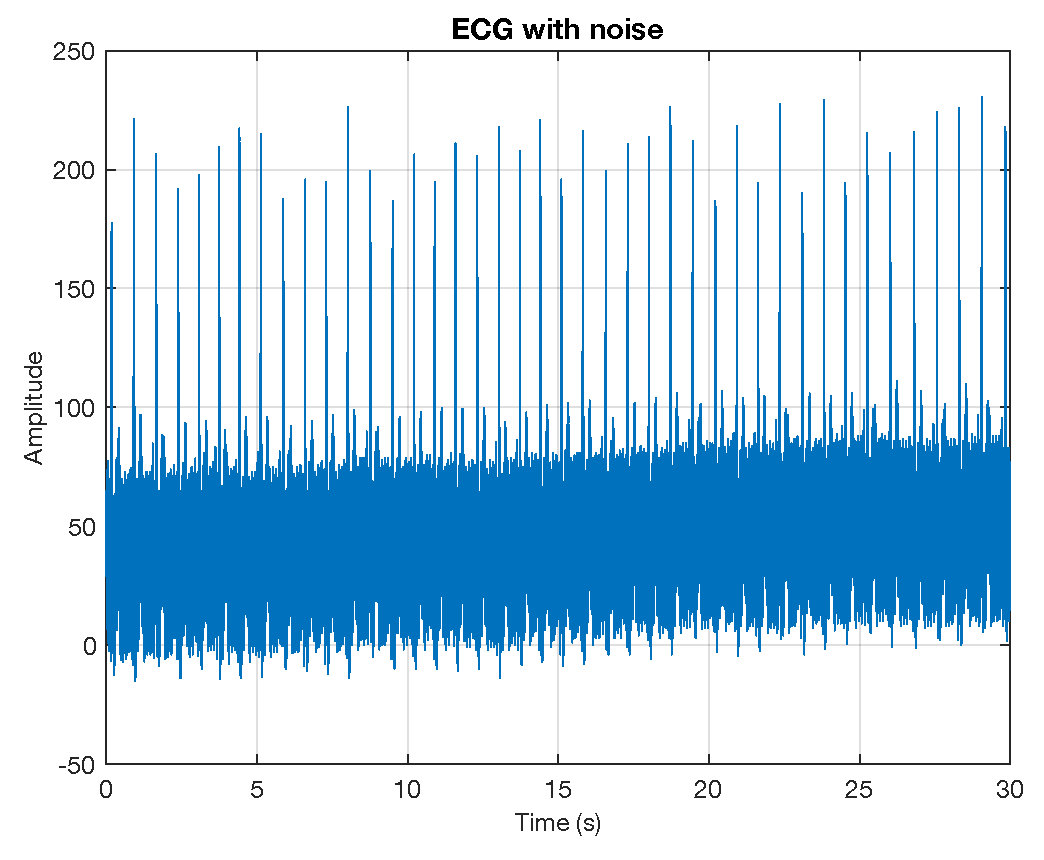
\includegraphics[width=0.9\textwidth]{resources/pdf/plot_a.pdf}
	    \caption{Whole signal as a function of time (in seconds)}
	    \label{fig:plot_a}
	\end{figure}
	\subsubsection*{Question (b)}
	Since the entire signal is not very visible, we only plot the signal between times 2 and 5 seconds (figure \ref{fig:plot_b}).
	\begin{figure}[H]
	    \centering
	    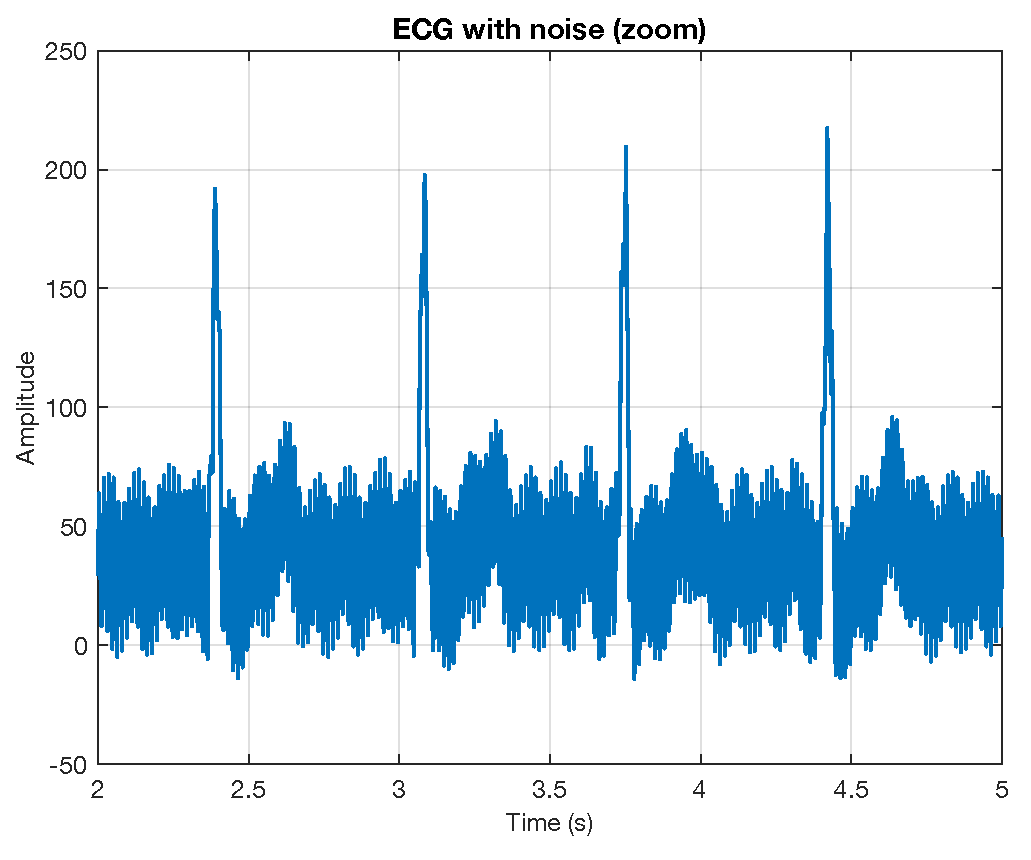
\includegraphics[width=0.9\textwidth]{resources/pdf/plot_b.pdf}
	    \caption{Signal between times 2 and 5 seconds}
	    \label{fig:plot_b}
	\end{figure}
	\subsubsection*{Question (c)}
	It is clearly observed that the signal is noisy. In order to identify the noisy frequencies, we plot the single-sided magnitude spectrum (thanks to the function \texttt{fft} of Matlab) of the signal (figure \ref{fig:plot_c}).
	\begin{figure}[H]
	    \centering
	    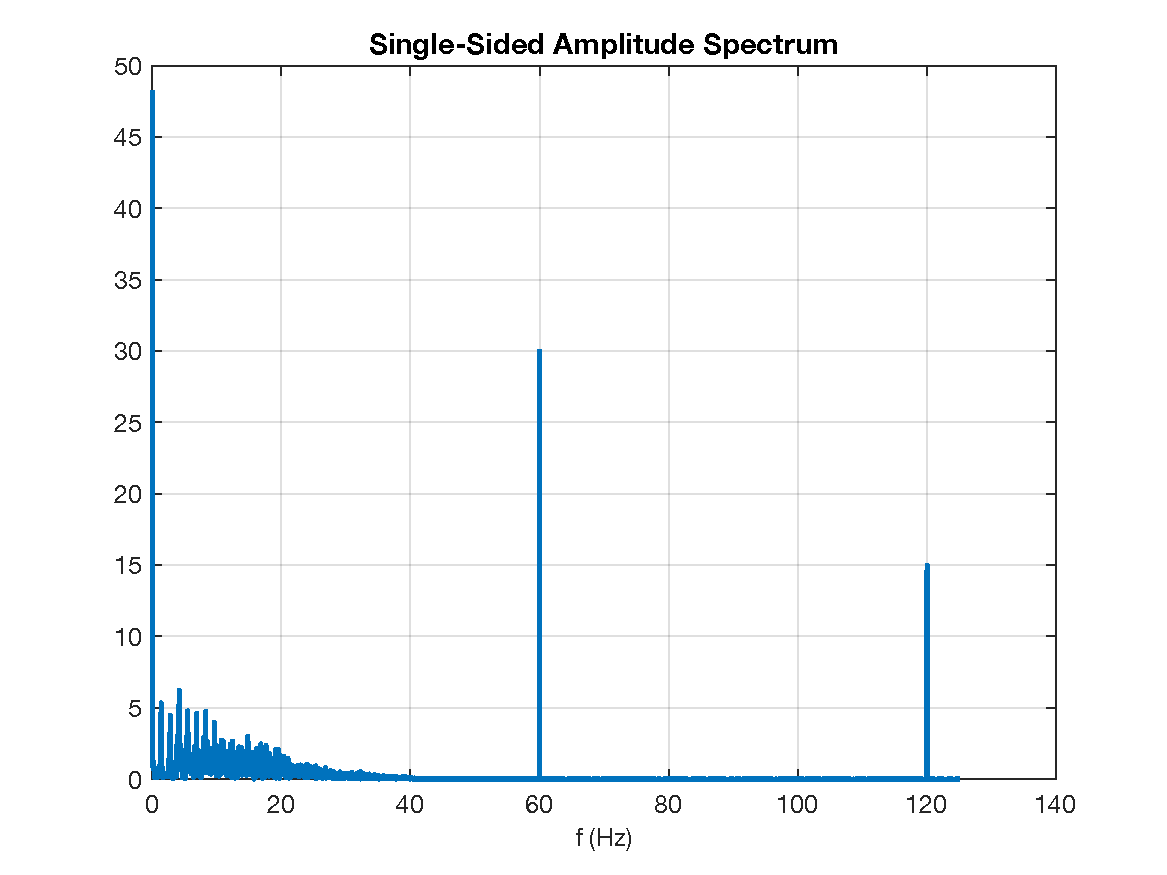
\includegraphics[width=0.9\textwidth]{resources/pdf/plot_c.pdf}
	    \caption{Single-sided magnitude spectrum of the signal}
	    \label{fig:plot_c}
	\end{figure}
	\subsubsection*{Question (d)}
	The two noisy frequencies are clearly identified by the two peaks: \SI{60}{\hertz} and \SI{120}{\hertz}.
	\subsubsection*{Question (e)}
	Both signals (noisy and non-noisy) are shown in figure \ref{fig:plot_e}.
	\begin{figure}[H]
	    \centering
	    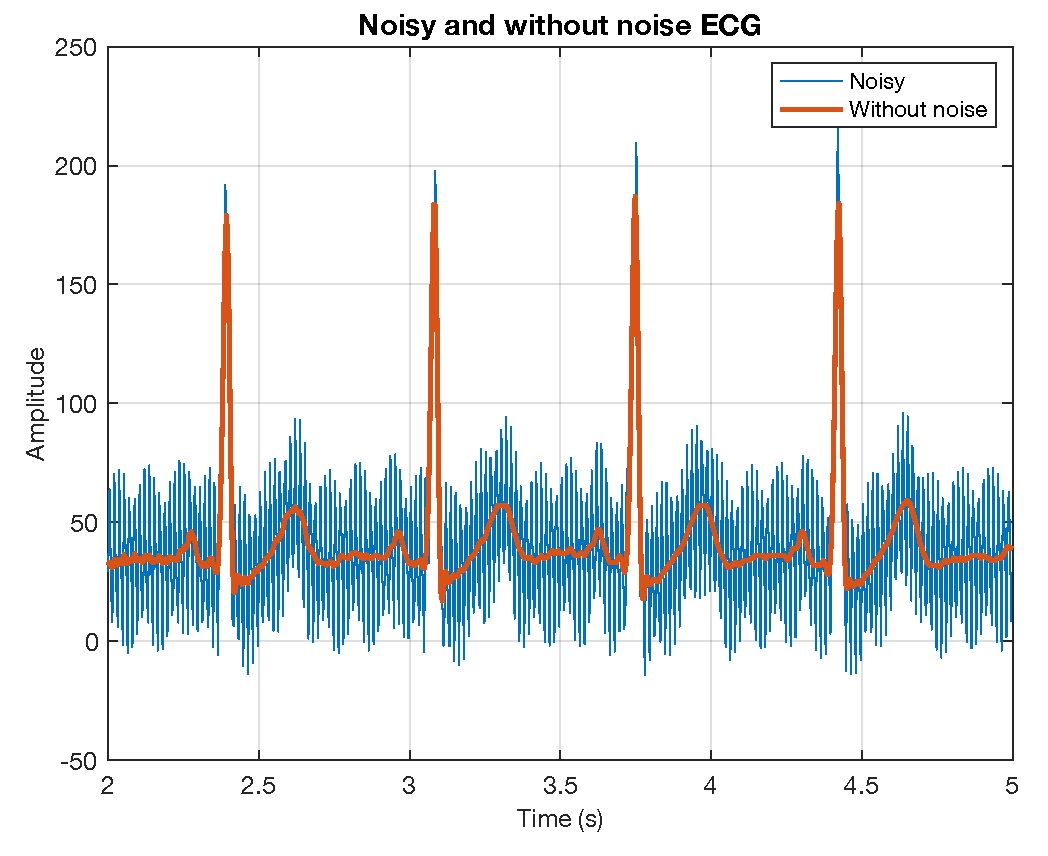
\includegraphics[width=0.9\textwidth]{resources/pdf/plot_e.pdf}
	    \caption{Noisy and original signal (from the second 2 to second 5)}
	    \label{fig:plot_e}
	\end{figure}
	\subsubsection*{Question (f)}
	We can create notch filters to filter the noisy frequencies. Indeed, a notch filter makes it possible to filter particular frequencies.\par
	In our case, we create two filters: one to filter the noise at \SI{60}{\hertz} frequency and the other to filter the noise at \SI{120}{\hertz} frequency.\par
	The filters were created with Matlab, with the procedure seen during the course.\par
	The two filters are shown in figures \ref{fig:filter_60} and \ref{fig:filter_120}. It can be seen that the magnitude response is effectively very low at \SI{60}{\hertz} and \SI{120}{\hertz} respectively (the filters therefore make it possible to remove the components at these frequencies).\par
	The x-axis is expressed in $\pi$ rad/sample. However, it is very simple to do the conversion and to find that one falls well on \SI{60}{\hertz} and \SI{120}{\hertz} respectively :
	\begin{align*}
	    \frac{\SI{60}{\hertz}}{F_{sample}/2} &= \frac{60}{125} = \num{0.48}\quad\pi\text{ rad/sample}\\
	    \frac{\SI{120}{\hertz}}{F_{sample}/2} &= \frac{120}{125} = \num{0.96}\quad\pi\text{ rad/sample}\\ 
	\end{align*}
	The phases of the filters are linear, they do not deform the signal.\par
	Applying these two filters in series, we can find the original signal, non-noisy.
	\begin{figure}[H]
	    \centering
	    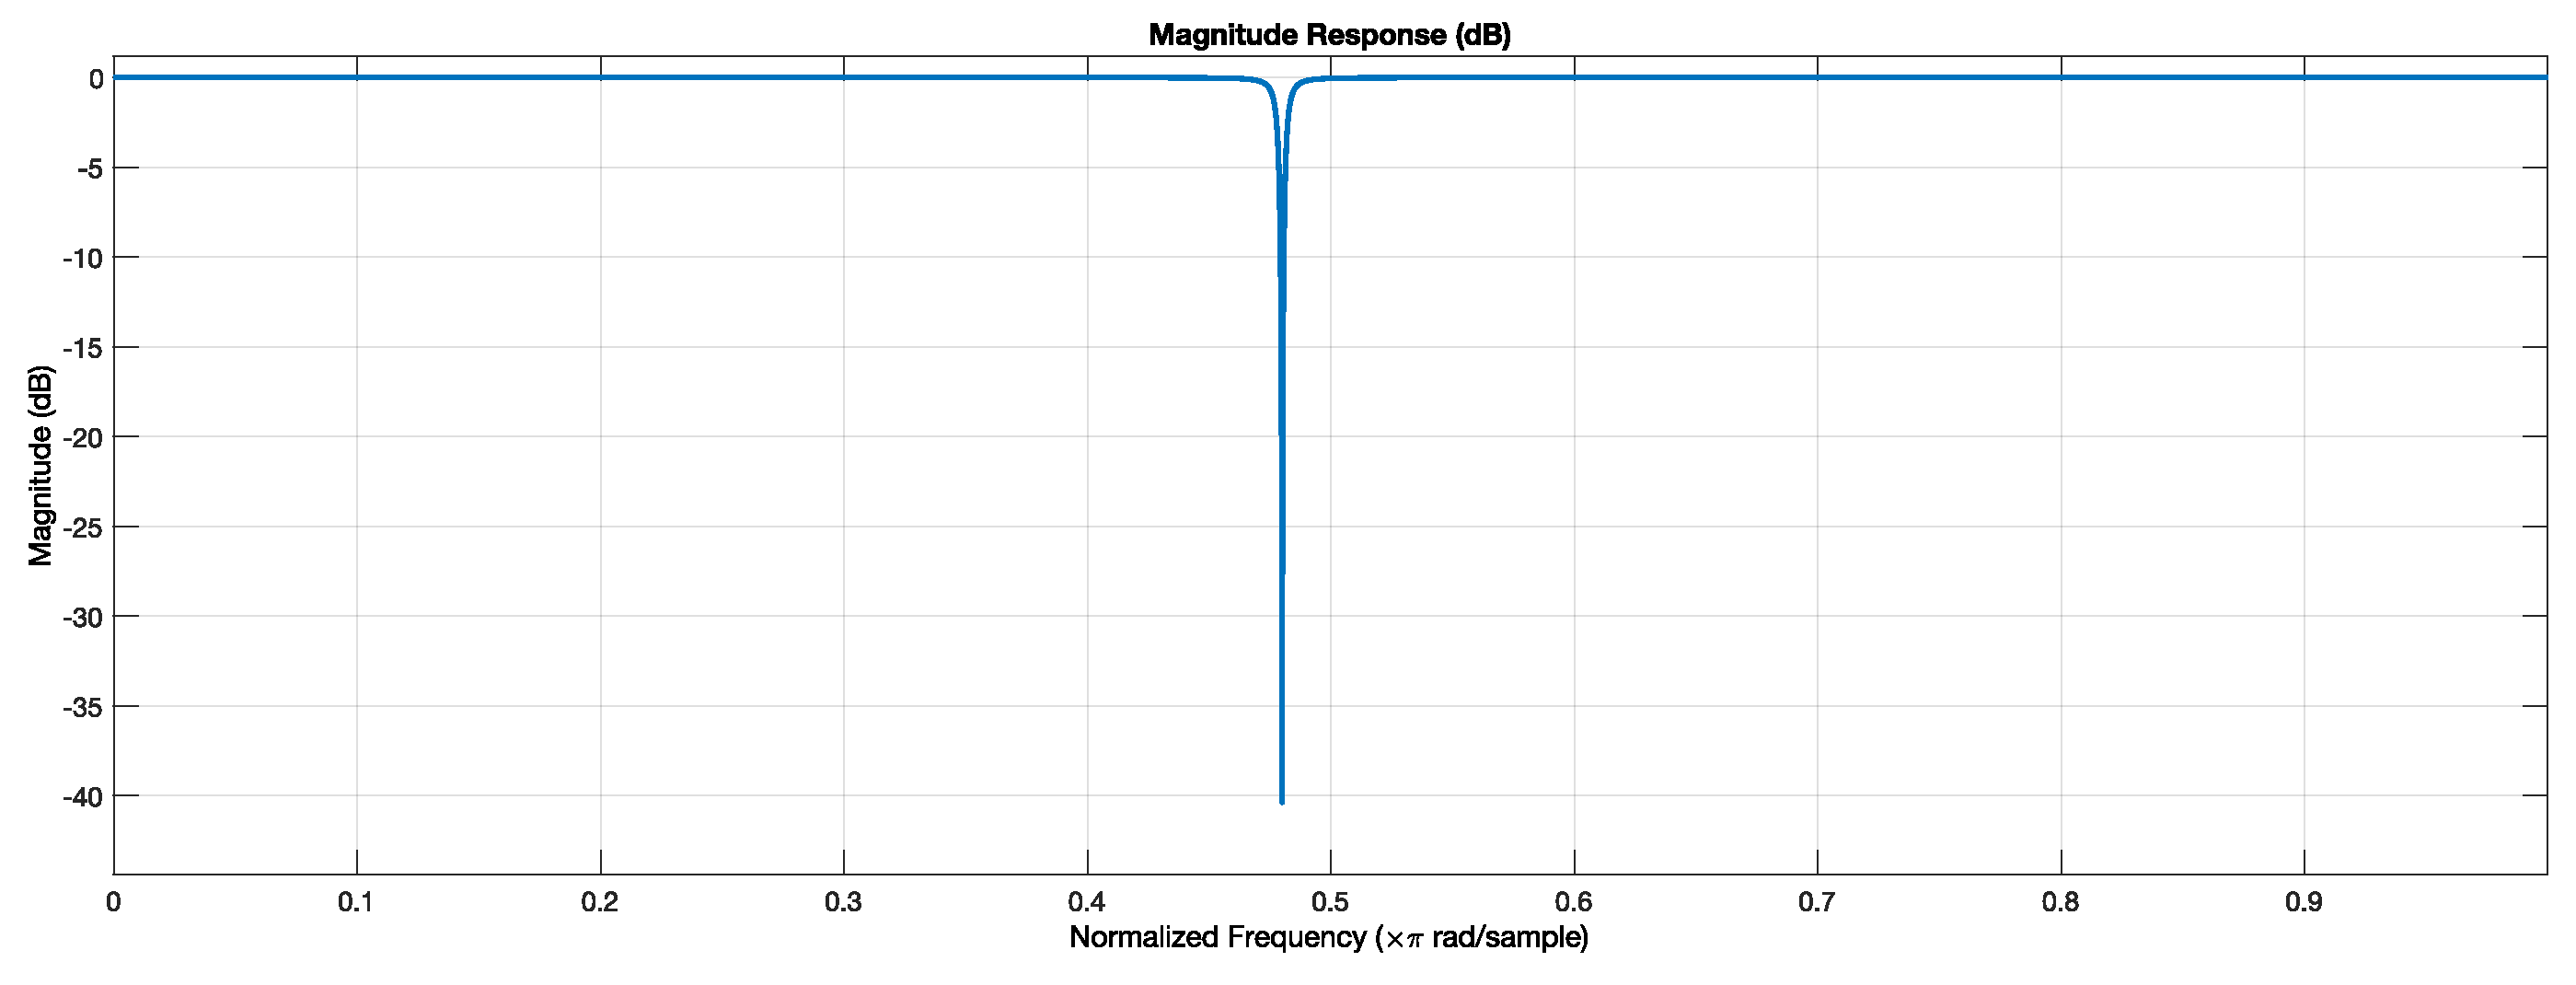
\includegraphics[width=1\textwidth]{resources/pdf/filter_60.pdf}
	    \caption{Magnitude response of the notch filter (\SI{60}{\hertz})}
	    \label{fig:filter_60}
	\end{figure}
	\begin{figure}[H]
	    \centering
	    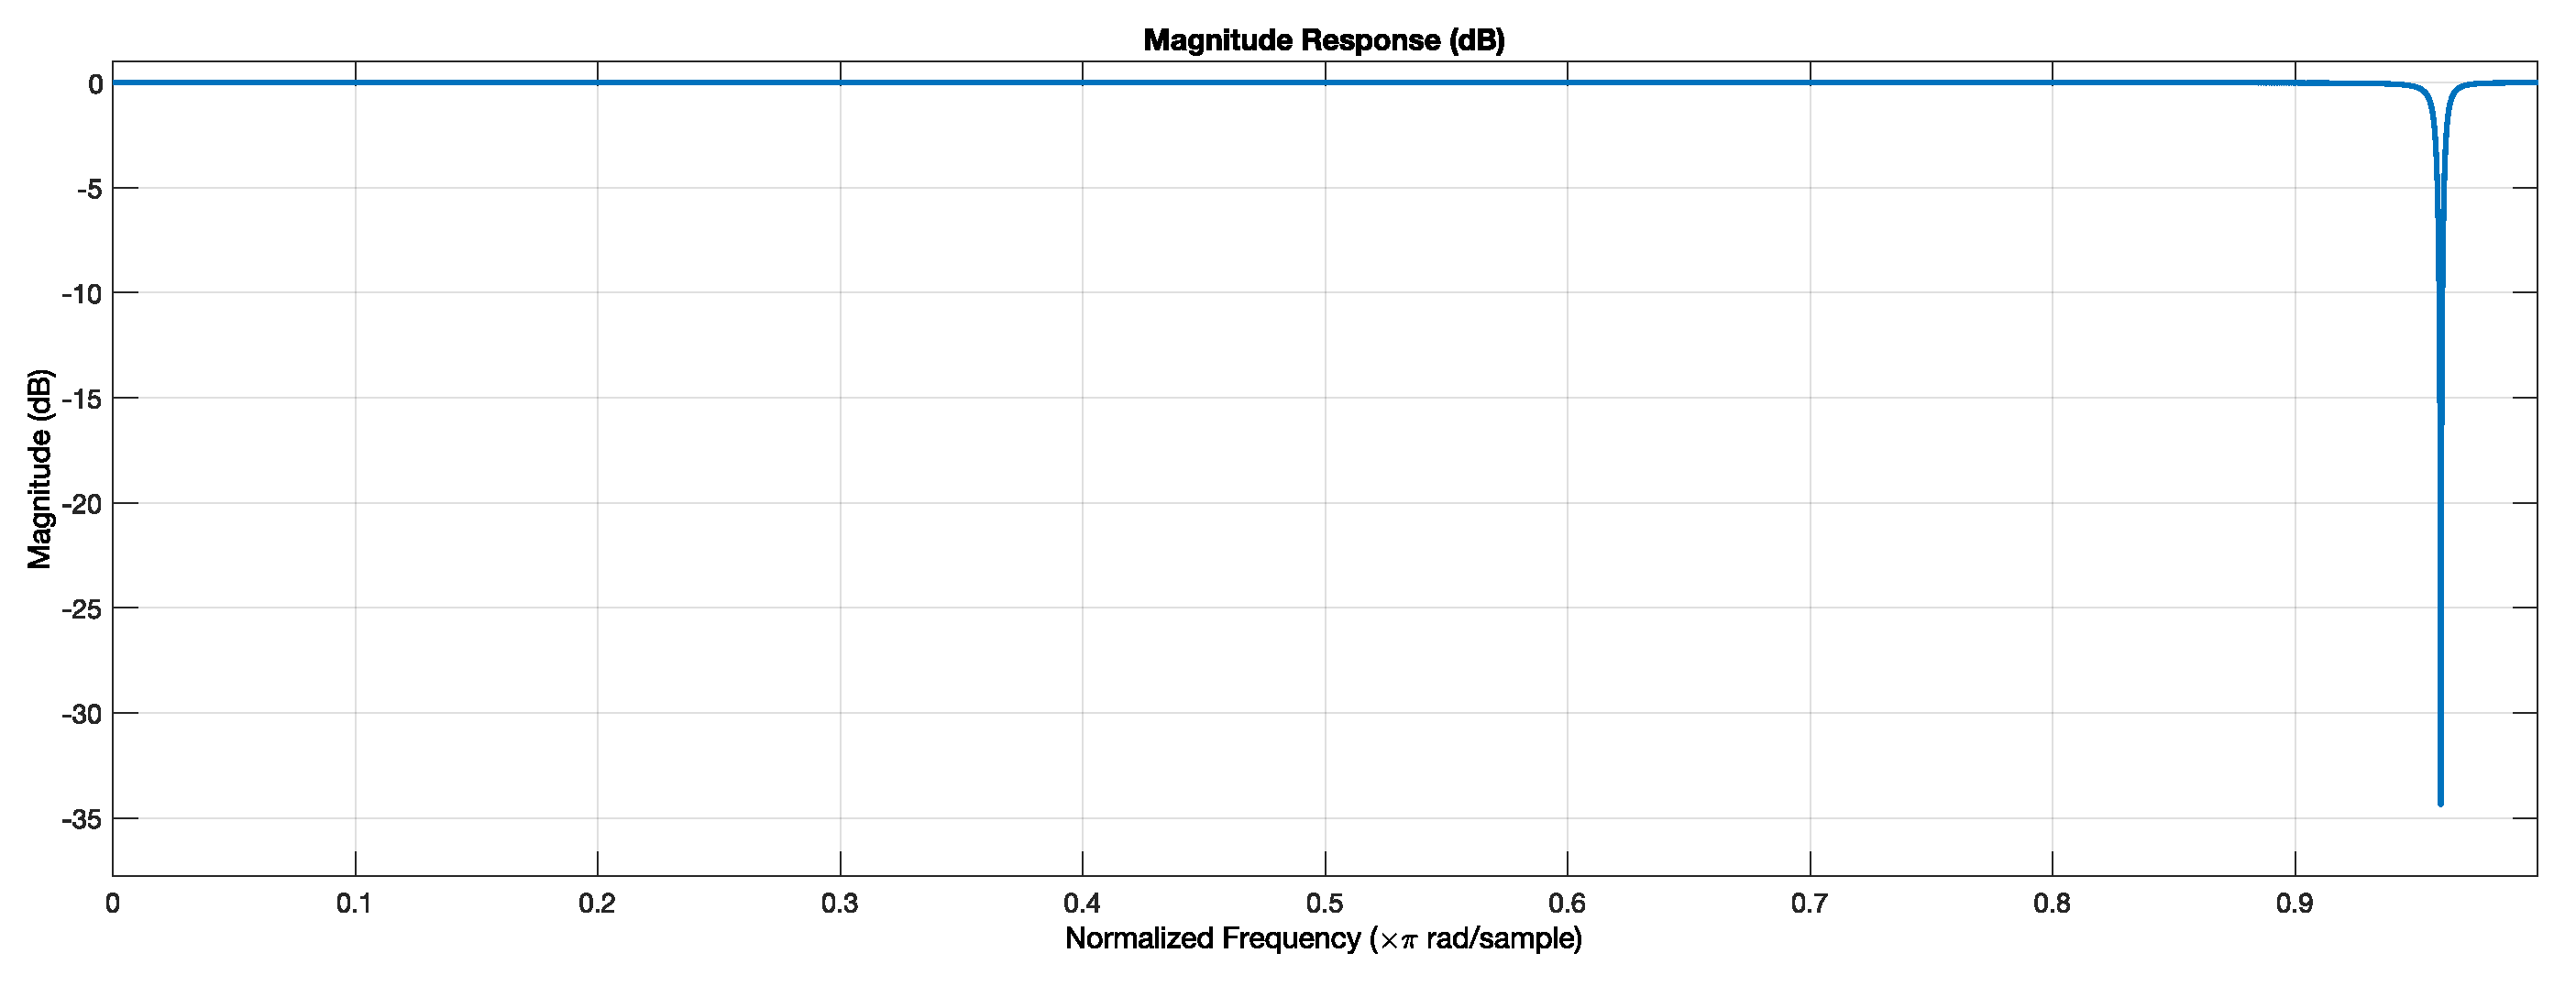
\includegraphics[width=1\textwidth]{resources/pdf/filter_120.pdf}
	    \caption{Magnitude response of the notch filter (\SI{120}{\hertz})}
	    \label{fig:filter_120}
	\end{figure}
	\newpage
	\appendix
	\section{Matlab code}
	\lstinputlisting[style=NFmatlab, caption={Elimination of noise on the signal \texttt{hw2\_electrocardiogram.mat}.}]{resources/m/Q1.m}
\end{document}
